\documentclass[12pt,oneside,final]{siuethesis}
\usepackage{microtype} % (optional) for more beautiful typesetting
\usepackage{graphicx} 
\usepackage{hyperref} %makes links clickable
\hypersetup{colorlinks,citecolor=black,filecolor=black,linkcolor=blue,urlcolor=black} %good for electronic copy
\hypersetup{colorlinks,citecolor=black,filecolor=black,linkcolor=black,urlcolor=black}%required for paper graduate school copy
%\usepackage[alphabetic]{amsrefs} %required if using amsrefs, comment out if using bibtex
\usepackage{fixltx2e}
\usepackage{amsmath}
\usepackage{epsf}
%\usepackage{float}
\usepackage{caption}
\usepackage{subfig}
%\usepackage{subcaption}
\usepackage{listings}
\usepackage{rotating}
\usepackage{tabularx}

\usepackage{multirow}

%% controls numbering of theorems
%% this can be configured to your advisor's taste
\newtheorem{theorem}{Theorem}[chapter] %theorem number resets each chapter
\newtheorem{conclusion}[theorem]{Conclusion}
\newtheorem{condition}[theorem]{Condition}
%% conjectures, corollary, defn, etc. numbered sequentially from beginning of chapters
\newtheorem{conjecture}[theorem]{Conjecture} 
\newtheorem{corollary}[theorem]{Corollary}
\newtheorem{example}[theorem]{Example} 
\newtheorem{lemma}[theorem]{Lemma}
\newtheorem{proposition}[theorem]{Proposition}
\newtheorem{solution}[theorem]{Solution}
\theoremstyle{definition}
\newtheorem{definition}[theorem]{Definition}


\author{Bryan Orabutt}
\title{Design and Analysis of a Mult-Channel Discriminator Integrated Circuit for Use in Nuclear Physics Experiments}

%%\advisor{John Q.\ Faculty} %% or 
\advisor{Dr.}{George L. Engel}
\secondreader{Dr.}{Bradley Noble} %% or \secondreader{Dr.}{Karl Gauss}
\thirdreader{Dr.}{Timothy York}
%\fourthreader{Karl Gauss, Sr.}
%\fifthreader{Karl Gauss, Sr.}
%\secondadvisor{Karl Gauss} %if you haves two advisors (rare) then use this line also and pass the option `twoadvisors' to the class
%\abstracttext{Chairperson: The Honorable Jill Smith} %optional -- you can use this to override the text on the abstract page; the grad school default is built-in
\submitdate{August, 2018} %date the month/year submitted to grad school, use a comma between
\copyrightyear{2016} %optional, but required if copyrighted

%% all of these are optional; defaults are shown
\major{Electrical Engineering} 
\degree{Master of Science} %can be used to specify M.A., etc.
\highestdegree{Master of Science} %used if the author already has another graduate degree
\department{Electrical and Computer Engineering} 
%\departmentname{Department}
%\refname{REFERENCES} 

%\captionsetup{width=0.7\textwidth}

\begin{document}
\maketitle 

\frontmatter %signals single spacing/roman numeral pagination

\copyrightpage %optional

% ^^^^^^^^^^^^^^^^^^^^^
% ABSTRACT
% ^^^^^^^^^^^^^^^^^^^^^

\begin{abstract}

This thesis documents the design, analysis, and simulation of a multi-channel integrated circuit (IC) consisting of 16 channels of constant fraction discriminators for use in Nuclear Physics experiments
document.  

\end{abstract}


% ^^^^^^^^^^^^^^^^^^^^^^^^^^^^^^^^^^^^^^^
% ACKNOWLEDGEMNTS
% ^^^^^^^^^^^^^^^^^^^^^^^^^^^^^^^^^^^^^^^^


\begin{acknowledgements}

I  would  like  to thank  Dr.  Lee  Sobotka  and  Mr.  Jon  Elson,  department  of  chemistry, 
Washington  University  Saint  Louis,  for  their  help  during  the  various  stages  of  this  project. 
My  special  thanks  to  the  faculty  and  staff  of  ECE  department  for  their  direct  and  indirect 
support without which I simply could not have progressed with my work. 



\end{acknowledgements}

\tableofcontents

\cleardoublepage %cause correct numbering of list of figures

\acknowledgements

\cleardoublepage

\listoffigures %print list of figures page

\cleardoublepage

\listoftables

\mainmatter %signals single spacing/arabic numeral paginations

% ^^^^^^^^^^^^^^^^^^^^^^^^^^^^^^^^^^^^^^^^^^^^^^^^^^^^^^^^^
%  CHAPTER 1
% ^^^^^^^^^^^^^^^^^^^^^^^^^^^^^^^^^^^^^^^^^^^^^^^^^^^^^^^^^

\chapter{INTRODUCTION}  %% chapter titles must be typed in all caps to conform with regulations

\section{Research Background}

\section{PSD8C IC}

Often in nuclear physics experiments the type of incident radiation must be classified, the energy of the particle must be determined, and the position of interaction within the detector must be estimated. This thesis presents design considerations for several systems that use gated integrators to extract the above information from the pulse. Since the performance of such systems depends upon the signal-to-noise ratio (SNR) of the integrators, an analysis of the SNR characteristics of a gated integrator is presented.  A particle identification (PID) system employing pulse-shape discrimination (PSD) is
highlighted. The proposed system makes use of a newly developed multi-channel integrated circuit (PSD8C). 

We demonstrate that the PID system will work well with both fast and slow detectors, such as organic liquids (e.g. BC 501) and CsI(Tl) scintillation detectors, respectively. For liquid scintillation detectors with a full scale energy range of 10 MeVee,
simulation shows a discrimination threshold (1 percent error of misclassification) of 1.44 MeVee (dynamic range of 17 dB). For CsI(Tl) scintillation detectors with a full scale energy range of 100 MeV, simulation shows a discrimination threshold of 1.55 MeV(dynamic range of 36 dB). 

%Pulse data from an experiment using a prototype CsI(Na) detector was also analyzed and used to generate an energy spectrum. The energy spectrums for a “noise-free” and  “noisy” (additive noise consistent with the PSD8C chip) system were compared. As these pulse data were collected with 137Cs (662 keV) and 60Co (1173 and 1332 keV) gamma-ray sources, the generated spectrum contained three Gaussian peaks corresponding to the photopeaks. The effect of the chip’s noise is not significant. The width of the first Gaussian increased from 5.68\percent to 6.34\percent. The second increased in width from 4.37\percent to 4.58 \percent while the third increased in width from 4.20\perecent to 4.24\percent. This work was initiated by the heavy-ion nuclear chemistry and physics group at Washington University in Saint Louis and is funded by NSF grant \#06118996.
%

%The thesis presents the design, simulation, and layout of an eight channel integrated circuit (IC) for use in nuclear physics experiments where particle identification, total pulse height, and relative timing information is needed.  The design employs a technique known as pulse shape discrimination (PSD) to classify the incident radiation.  Each of the eight channels is composed of a time-to-voltage converter (TVC) with two time ranges (0.5 sec, 2 sec) and three sub-channels.  Each of the sub-channels consists of a gated integrator with 8 programmable charging rates and an externally programmable gate generator that defines the start (with 4 time ranges) and width (with 4 time ranges) of the gate relative to an external discriminator signal.  The chip supports 3 triggering modes. 
%The IC produces four sparsified analog pulse trains (3 integrator outputs and 1 TVC output) with synchronized addresses for off-chip digitization with a pipelined ADC. The micro-chip, christened PSD8C, with two bias modes occupies an area of approximately 2.8 mm x 5.7 mm and has an estimated power dissipation of 135 mW in the high-bias mode.  T
%
%
%
%
%
%As part of a joint research effort, Washington University and Southern Illinois University Edwardsville are developing systems employing multiple charge integration for the detection of ionizing radiation.  The current objective of the research is to produce a micro-chip capable of particle identification that will complement an existing (shaped and peak-sensing) analog chip called HINP16C (Engel et al., Nucl. Instru. Methods A573, 418-426 (2007)).  Much of the work presented in this thesis was used to guide the design of this new chip, christened PSD8C (Pulse-Shape Discrimination – 8 Channels).
%A detailed description of the PSD8C chip can be found in a companion thesis written by another graduate student, Justin Proctor.  A brief description of the PSD8C chip is provided here.  Each of the eight channels is composed of a time-to-voltage converter (TVC) with two time ranges (0.5 µsec, 2 µsec) and three sub-channels.  Each of the sub-channels consists of a gated integrator with 8 programmable charging rates and a pair of externally programmable gate generators that define the start (with 4 time ranges) and width (with 4 time ranges) of the gate relative to an external discriminator signal.  The chip supports 3 triggering modes.
%PSD8C produces four sparsified analog pulse trains (3 integrator outputs and 1 TVC output) with synchronized addresses for off-chip digitization with a pipelined ADC.  The PSD8C chip with two biasing modes occupies an area of approximately 2.8 mm x 5.7 mm and has an estimated power dissipation of 135 mW in the high-bias mode.  The chip is to be fabricated in the AMIS 0.5-micron NWELL process (C5N) in early 2008.  While the chip was designed to perform particle identification using pulse-shape discrimination (PSD), it may also be used to obtain total pulse-height information.  It will be able to work with many different types of detectors.
%In a radiation detection system, detectors are used to sense radiation.  When struck by a particle, a detector will produce a pulse.  Encoded in the pulse-shape is information about the incident radiation including the pulse-height, particle type, and/or position of interaction within the detector.  While the parameters may be extracted in many different ways, this thesis analyzes analog-based systems that employ multiple charge integration to extract the information.  This method is not only effective but produces systems that are small (and relatively speaking, inexpensive).  Alternative DSP-based approaches can claim neither of these advantages.
%In the remainder of this chapter, three examples of systems that employ multiple charge integration will be described.  The three systems are intended for use in three different types of applications:
%1.	Applications requiring total pulse-height information 
%2.	Applications requiring particle identification using pulse-shape discrimination
%3.	Applications requiring information regarding position within detector where a particle deposited its energy
%The first two of these systems will be analyzed, and the performance, when implemented using the PSD8C IC, will be presented.  The third, since it has not been fully developed will only be discussed briefly here in Chapter 1.  Before discussing these three systems, some additional background material explaining how detectors and light sensors work will be provided.  It is hoped that this information will make it easier for the reader to understand the models presented in Chapter 2 of this thesis.
%
%Detectors
%Scintillation detectors are commonly used in the detection of ionizing radiation.  They work by converting a fraction of the deposited energy into visible light.  The detector is coupled to either a photomultiplier tube or a photodiode.  Most of the energy deposited in a scintillator ends up being degraded into vibrational phonons in the crystal, i.e. the bulk of the energy is converted to heat.  However, a fraction (~ 10% in bright scintillators) is converted into visible photons.  The total number of these visible photons (total time integral) is proportional to the energy deposition in the scintillator.  In many crystals, the time dependence of the pulse shape depends on the type of ionizing radiation and thus a pulse-shape analysis yields the particle type (gamma-ray, electron, proton, alpha-particle, etc.).
%There are two different types of scintillating material:  organic and inorganic.  Organic scintillators are either liquid or solid (either crystal or amorphous plastic for the latter) and can take on many different shapes and sizes.  One of the main advantages of organic scintillators is that they have fast decay times.  This means that the time of interaction can be determined with better resolution.  Inorganic scintillators are always crystals.  They can have a very high light yield, and long, short, or a mixture of decay times.  Three of the most common inorganic scintillators are NaI(Tl), CsI(Tl), and CsI(Na) (Knoll 221-222, 235).
%The light output of many scintillators is nonlinear in the amount of light they produce per unit energy.  As Birks first suggested, this is primarily due to quenching which degrades the light output (Knoll 227).  It is therefore convenient to measure the light output (or pulse-height) in the equivalent pulse-height that electrons would produce, the electron equivalent energy (i.e. MeVee).
%
%Light sensors
%The light from a detector is converted to an electric charge using a light sensor.  Two light sensors that are typically used are a photomultiplier tube and a photodiode.  A photomultiplier tube (PMT) consists of a photocathode followed by a cascade of dynodes and terminated by an anode.  When a photon of light enters the photocathode, it may interact to produce an electron.  The probability of converting the visible photon into an electron at the photocathode is known as the quantum efficiency.
%Photomultiplier tubes typically have low quantum efficiency, in the range of 20%.  This low quantum efficiency degrades the energy resolution which is ultimately determined by counting (Poisson) statistics of the primary photoelectrons generated at the cathode.  These primary electrons then go through the cascade of dynodes which will multiply them.  When an electron hits a dynode, several more electrons are produced.  Since there is a cascade of dynodes, the multiplication occurs many times giving several orders of magnitude of gain.  This will occur in a highly linear fashion (if the dynode string is “stiff”, i.e. the transient charge is small compared to the stored charge on the capacitors attached to each dynode).  The resulting electrons are then collected at the anode terminal.  The photomultiplier tube is an exceedingly low-noise device which is one of its main advantages (Knoll 265-273).
%A photodiode is a semiconducting device with a p-n junction that is sensitive to light.  When photons strike the p-n junction, it will then generate current (Streetman and Banerjee 398).  The classic photodiode has high quantum efficiency but no electron multiplication.  A separate charge-sensitive amplifier must be used to generate a detector signal.  The main advantage of photodiodes is that they are smaller than PMT’s, an advantage which is sometimes paramount.  As CSA’s are generally far noisier than a PMT, photodiodes generally do not perform as well as a PMT (Knoll 287-288).
%
%Example Systems That Employ Multiple Charge Integration
%Systems employing multiple charge integration can be used for many different applications.  Some applications may need to get total pulse-height information whereas others may require particle identification (PID) or information regarding the position within the detector where the energy was deposited.  Three example systems will be discussed.
%The first system used multiple charge integration to get total pulse-height information and to tag pile-up.  The second system used pulse-shape discrimination (PSD) to identify the type of particle as well as the deposited energy.  The third system will use (what we like to refer to as) an analog-assisted DSP (AA-DSP) technique to gather more detailed pulse-shape information.  In the later case, when the data originates from a large volume solid-state Ge detector, the shape analysis will yield the position of interaction in the detector as well as deposited energy and timing information.  Most of the attention in this thesis will be directed at the first two systems, since at this point in time the third system has not yet been fully developed.
%
%Total pulse-height information using the high resolution scintillation array (HiRSA)
%Multiple charge integration can be used to get total pulse-height information and to detect and tag pile-up.  A single integrator can be used to extract energy information by integrating over the entire (or a large percentage) of the pulse.  If a second integrator is used to integrate over a different region, then the ratio of the two integrators can be used as a means to detect pile-up.  Simulations were done on real digitized pulse waveforms from a CsI(Na) detector which is the prototype for a new detector project at the National Superconducting Cyclotron Laboratory (NSCL) at Michigan State .  In this section, I describe the reason for this new detector system, the working elements, and provide a few words about alternative electronics for this application.
%Much of present day nuclear physics concerns the structure of nuclei removed from beta-stability.  The study of the properties of such nuclei requires reactions to be preformed with them.  The NSCL is a facility devoted to creating beams of these unstable nuclei.  What this really means is all experiments are secondary beam experiments.  A primary stable beam slammed into a stable target.  One or more of unstable products of this primary reaction are selected to make a secondary beam which is used, together with a secondary target, to initiate a second reaction.  While the nuclei in the secondary beam are unstable, they have lifetimes longer than 1 ms.  This is plenty of time for electrostatic means of generating a beam (by say selection on magnetic rigidity and velocity or specific energy loss) which works on times scales of less than 1 µs.
%The simplest secondary reaction would be a “Coulomb excitation” reaction.  In this process the unstable nuclei are excited by the time varying Coulomb Field as it flies closely by a nucleus of an atom in the secondary target.  Once excited, it will decay by emitting gamma-rays, the energies of which tell you about the excited quantum states of the unstable nucleus.  To make this experiment work, one needs a gamma-ray detector with high efficiency (as the secondary beams are generally very low in intensity) and with as high resolution as possible.  The first such array at the NSCL was provided by Washington University.  This was a set of long cylindrical NaI(Tl) detectors salvaged from an decommissioned PET.  The second, was a larger array of NaI(Tl) from Argonne National Laboratory.  The third was a large array of solid state Ge detectors.  The Ge detectors have outstanding energy resolution but very poor efficiency.  In an effort to complement the Ge array, the staff at the NSCL proposed and were approved to build a 192 element CsI(Na) scintillation array.  The (tentative) name of this device is:  High Resolution Scintillation array (HiRSA).
%CsI(Na) is a scintillator with a brightness (~ 40 visible photons per keV deposited) very similar to NaI(Tl) but with a better match to peak quantum efficiency of photocathodes used in PMT’s.  The channel count (~ 200) is sufficiently large to warrant careful consideration of cost of the electronics per channel.  However, one must not sacrifice energy resolution and should maintain the ability to identify pile-up events.
%The detectors in the array are either square (3”x3”x3”) or rectangular (2”x2”x4”) with either the 3”x3” or 2”x2” face attached to the PMT.  By mid 2007, the NSCL had a prototype and had conducted source tests with both digital and conventional electronics.  For testing the DSP, they collected (and stored) digitized wave forms (10 ns intervals) from one of the prototypes.  The source tests used weak 137Cs (662 keV) and 60Co (1173 and 1332 keV) gamma-ray sources.  Weak sources were used to minimize pile-up for these first tests.  Due to the fact that weak sources were used, natural background gammas from 40K (1460 keV) and 226Ra (609 keV) were detected.
%While the NSCL was funded (by the NSF) for the physical device, they were not given any funds for the electronics.  The initial cost estimate for a fully digital system was close to 200 k$ (~ 900 $/ch).  On top of this, FPGA development would need to be done.  The full cost of implementing our PDS system (post development) was estimated to be only 30 k$.  This factor of 7 reduction (from DSP to chip analog – with some signal shape analysis) is similar to what we have found in other applications and a major reason why this chip development was undertaken.  (Keep in mind that the development of the DSP is very large and also largely borne by the federal government in the form of grants to universities, national laboratories and private companies.)
%
%Particle identification using pulse-shape discrimination (PSD)
%Particle identification of nuclear radiation is typically done using pulse-shape discrimination (PSD).  There are several ways in which this can be accomplished:
%1.	“Sensing differences in the decay times of pulses”
%2.	“Integrating pulse charge over different time intervals”
%3.	“Digital capture and shape analysis of pulses”
%The first method works by filtering the pulse through a shaper to produce a “bipolar pulse”.  The shape of this bipolar pulse and its zero-crossing depends on the pulse shape and decay time.  Since different particles will have different pulse shapes and decay times, the time difference between the zero-cross and the start of the pulse will change depending on the type of particle that struck the detector (Bryan et al. 1).
%The second method works by integrating the pulse over various time intervals.  The results of the integrations depend on both the deposited energy and the particle type.  To discriminate between particles, the integration needs to be normalized by looking at the ratio between two integrators.  There is usually a fast and slow component in the pulse waveform that depends on both the deposited energy and the particle type.  Therefore, if one were to capture these two components and look at their ratio (which is actually a function of the deposited energy), then the particle type can be determined (Bryan et al. 1).
%The third method works by using high-speed analog-to-digital flash converters to digitize each pulse and then do a complete “shape analysis”.  The shape analysis is done “off-line [using a computer rather than in an analog fashion] to determine particle type, energy, and timing information” (Bryan et al. 1-2).
%Although the main purpose of pulse-shape discrimination (PSD) is for particle identification, we will also show that this pulse-shape information can be used to tag and perhaps correct pile-up events.  Typically PSD is done using a detector, a constant-fraction discriminator, and multiple gated integrators.  Crucial to PSD is the photodetector’s electronics noise.  A good detector should have a high light yield and very little electronic noise.  These conditions minimize the detection threshold for discriminating between particles.  One way to determine the effectiveness of a PSD system is to calculate a figure-of-merit (Marisaldi et al. 1917-1919):
% 	(1.1)
%In equation 1.1, r is the ratio between two integrators, Δr is the difference in the ratios for two particles and σtot is the square root of the sum of the noise variances of the r distributions for the two particles.  The figure-of-merit allows us to judge the PSD system.  A high figure-of-merit will allow better particle discrimination.  There are two ways to increase the figure-of-merit.  One is to make Δr larger and the other is to decrease the noise is both r distributions.  This can be done by picking good integration regions and integration time constants.  Noise can also be improved by picking a good detector with a high light yield, and by reducing the electronics noise of the system.
%
%Positional information using analog-assisted DSP (AA-DSP)
%A future system is being planned that will get the position of interaction in the detector using an analog-assisted DSP approach.  Analog-assisted DSP is a mix between charge integration and traditional digital capture methods.  It utilizes multiple analog “round-robin” charge integrators to integrate under each region of a pulse.  Then using digital signal processing, the position of interaction in the detector, deposited energy, and timing information can be determined.  In order to characterize a pulse, there will be, for example, 12 fast charge integrators and 12 slow charge integrators.  The fast charge integrators are used to capture the fast rising portion of the pulse whereas the slow charge integrators are used to capture the slow decaying portion of the pulse.  An illustration showing the 12 slow charge integrators can be seen in figure 1.1.
% 
%
%Figure 1.1 Round-robin charge integrators used in AA-DSP
%
%Since this is a round-robin scheme, the 12 fast and slow charge integrators are continuously running.  However, when a new pulse arrives, a counter is started which will stop the round-robin integrators after 10 integrations have occurred past the arrival of the pulse.  The values of these integrators are then held until retrieved for off-line analysis.
%
%
%
%
%
%
%
%
%





\section{Need for an Integrated Circuit}

\section{Sample Applications}

\section{Features of CFD16C}

\section{Object and Scope of Work} 

% ^^^^^^^^^^^^^^^^^^^^^^^^^^^^^^^^^^^^^^^^^^^^^^^^^^^^^^^^^
%  CHAPTER 2
% ^^^^^^^^^^^^^^^^^^^^^^^^^^^^^^^^^^^^^^^^^^^^^^^^^^^^^^^^^


\chapter{SYSTEM ARCHITECTURE}

This chapter will attempt to describe the CFD16C integrated circuit at the system-level.  We will start with a detailed list of system requirements and then will describe the high-level architecture of the IC.

\section{System Specifications}
The success of our group over the past 20 years lies in the fact that in the close working relationship that the IC Design Research Laboratory at Southern Illinois University Edwardsville (SIUE) has had with the Nuclear Reactions Group at Washington University in St. Louis(WUSTL) led by Dr. Lee Sobotka.  The IC group here at SIUE and the Nuclear Reactions Group at WUSTL, after lengthy discussions, drafted the following specifications for the IC described here in this thesis.

\begin{itemize}
\item
The IC should support 16 detectors.
\item
It should support analog pulses of both polarities (relative to analog signal ground).
\item
It should accommodate analog exponentially shaped pulses with risetime constants ranging from 3 nsec to 100 nsec.
\item
It exhibit "excellent" walk and jitter characteristics for input pulse amplitudes ranging from 20 mV to 2 V. The adjective "excellent" will be quantified in a later chapter of this thesis.
\item
Pulse repetition rates up to 1 KHz must be accommodated.
\item
The discriminator in each of the 16 channels should be of the constant fraction type (CFD). In CFD discriminators an attenuated version of the input is subtracted from a delayed version of input waveform and the time at which the difference between the two is equal to zero is used to mark the pulse arrival time. This results in output timing signals independent of pulse amplitude.
\item
Each channel should have a leading-edge threshold. The threshold is programmed using a 4-bit digital value.
\item
While the chip must support signals with risetime constants ranging from 3 nsec to 100 nsec, performance will be optimized for the shorter time constants. 
\item
The output pulse width from a channel will be programmable (through an external analog control voltage) in the range of 10 nsec to 100 nsec.
\item
The analog supply voltage for the IC will be 5 Volts while all digital signals entering and leaving the IC will obey a 3.3 Volt standard.
\item
Power consumption of the 16 channel IC should not exceed 350 mW \emph{i.e.} 20 mW per channel with 30 mW budgeted for the circuits common to all channels. 
\item
The IC is not to occupy an area greater than roughly 2 mm x 3 mm.  The chip should be packaged in a 64-pin plastic package.  
\item
The chip should be fabricated in the AMS-AG, 0.35 micron CMOS process.  The targeted process supports two poly and 4 metal layers.  A high resistance poly layer is also available.
\end{itemize} 

\section{System Overview}


% ^^^^^^^^^^^^^^^^^^^^^^^^^^^^^^^^^^^^^^^^^^^^^^^^^^^^^^^^^
%  CHAPTER 3
% ^^^^^^^^^^^^^^^^^^^^^^^^^^^^^^^^^^^^^^^^^^^^^^^^^^^^^^^^^


\chapter{ELECTRICAL LEVEL DESIGN}

\section{Process Parameters}

\section{Common Channel}

\subsection{Configuration registers}

\subsection{Signal ground generator}

\subsection{Bandgap voltage reference}

\subsection{PTAT current reference}

\subsection{Zero-tempco current reference}

\subsection{Lockout DAC}

\subsection{Multiplicity output buffer}




\section{Discriminator Channel}

\subsection{Programmable Nowlin Circuit}

\subsection{Leading-Edge Detector}

\subsection{Zero-Cross Detector}

\subsection{Output One-Shot}


%silicon strip detector array shown in Figure~\ref{FIG:PACKAGED_PARTS}.
%\begin{figure}[htbp!]
%\centering
%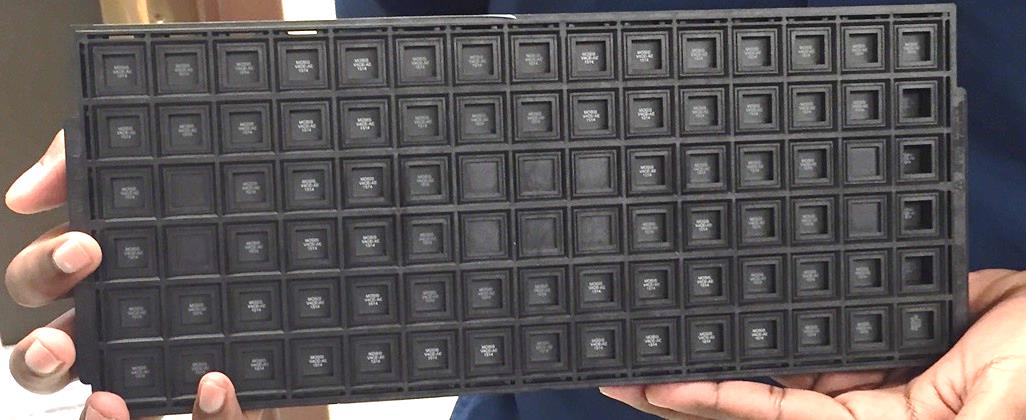
\includegraphics[scale=.4,keepaspectratio=true]{./ch3_figures/packaged_parts.png} 
%\caption{Custom Chip For Use With 
%Silicon Strip Detectors}
%\label{FIG:PACKAGED_PARTS}
%\end{figure}


% ^^^^^^^^^^^^^^^^^^^^^^^^^^^^^^^^^^^^^^^^^^^^^^^^^^^^^^^^^
%  CHAPTER 4
% ^^^^^^^^^^^^^^^^^^^^^^^^^^^^^^^^^^^^^^^^^^^^^^^^^^^^^^^^^



\chapter{SIMULATION RESULTS}



% ^^^^^^^^^^^^^^^^^^^^^^^^^^^^^^^^^^^^^^^^^^^^^^^^^^^^^^^^^
%  CHAPTER 5
% ^^^^^^^^^^^^^^^^^^^^^^^^^^^^^^^^^^^^^^^^^^^^^^^^^^^^^^^^^


\chapter{SUMMARY, COMCLUSIONS, AND FUTURE WORK}

\section{Summary}


\section{Conclusions}

\section{Future Work}

\references %single spacing / arabic numeral paginations, adds "REFERENCES" to table of contents

%%%% for bibtex

%If you want to use bibtex  use the following lines, where your .bib file is called 'yourbib.bib'

\bibliographystyle{apalike}
\bibliography{./orabutt_thesis}

% If you have only a single appendix, do it this way.

\multipleappendices
\lstset{
         language=C,
         basicstyle=\scriptsize\ttfamily,
         emptylines=0, 
         lineskip=1pt,
         %numbers=left,            
         numberstyle=\tiny,         
         stepnumber=2,              
         numbersep=5pt,             
         tabsize=3,                
         extendedchars=true,       
         breaklines=true,            
         commentstyle=\color{blue},
         keywordstyle=\color{red},
            frame=b,         
 %        keywordstyle=[1]\textbf,    
 %        keywordstyle=[2]\textbf,    
 %        keywordstyle=[3]\textbf,  
 %        keywordstyle=[4]\textbf,   \
         stringstyle=\scriptsize\color{green}\ttfamily, 
         showspaces=false,         
         showtabs=false,            
%         xleftmargin=17pt,
%         framexleftmargin=17pt,
%         framexrightmargin=5pt,
%         framexbottommargin=4pt,
         %backgroundcolor=\color{lightgray},
         showstringspaces=false           
 }


\end{document}
